This chapter describes the proposed approach for generating Puzzle Script levels and rules using different methodologies. This chapter is divided into two parts Level Generation and Rule Generation.

\section{Level Generation}
Level Generation is not an easy task specially when the game rules are not known before generation. Most of the previous work in the Puzzle Level Generation (refer to \chref{Chapter3}) was limited for generating levels for a specific game. Although some research suggested a general technique to generate levels, it is still based on designing a game specific fitness function. In this work, we suggest some global metrics for Puzzle Games that can help in generating levels with the minimum prior knowledge.\\\par

Our approach relies heavily on the understanding of the current game rules and some prior knowledge about Puzzle Script language. \figref{levelGenBlockDiagram} shows a high level block diagram of the system. The following subsections will describe each block in details.

\gfigure{High level system block diagram for Level Generation}{levelGenBlockDiagram}{width=5.5in}{Images/levelGenBlockDiagram}

The system starts by analyzing the current game rules using a Rule Analyzer. The Rule Analyzer utilizes some basic information about Puzzle Script rules to understand the importance of each game object and its basic functionality.\\\par

The output of the Rule Analyzer (Object Features) and the Level Outlines are fed to a Level Generator. The Level Generator is responsible for generating initial level layouts. It utilizes the Object Features to insert game objects at suitable positions in the Level Outlines. Level Generator uses two different approaches: a Constructive Approach and a Genetic Approach. The Constructive Approach is faster in generation but produce less diverse levels, while Genetic Approach requires more time but gives access to a vast majority of levels.\\\par

The generated levels are subjected to a Level Evaluator. The Level Evaluator uses an automated player to play the generated levels. Based on the result of each play, the Level Evaluator gives a score to the level based on some heuristic measures. These measures make sure that the resulting level is playable and challenging.\\\par

In case of the Constructive Approach, the system selects the best scored levels to output them, while the Genetic Approach enhances the output levels using GA.

\subsection{Rule Analyzer}\seclbl{ruleAnalyzer}
The Rule Analyzer is the first module in our system. It analyzes game rules and extract some useful information about each object. The extracted information is fed to the Level Generator and the Level Evaluator. Each object is assigned:
\begin{itemize}
	\item \textbf{Type:} Object type depends on its presence in the Puzzle Script file. There are 4 different types:
	\begin{itemize} \itemsep0pt \parskip0pt \parsep0pt
		\item \textbf{Rule Object:} Any object that appears in a rule is defined as a rule object. Rule objects are essential for rules to be applied.
		\item \textbf{Player Object:} It is defined by name "Player" in the Puzzle Script. It is the main game entity. It can move freely without any restriction. Any level must have at least 1 player object. Player object is a Rule Object as well.
		\item \textbf{Winning Object:} They are objects appearing in the winning condition. At least one of them is a Rule Object or a Player Object.
		\item \textbf{Solid Object:} All objects that does not appear in any rule but on the same collision layer with a Rule Object.
	\end{itemize}
	\item \textbf{Subtype:} each Rule Object is assigned a Subtype based on its presence in game rules. These subtypes are:
	\begin{itemize} \itemsep0pt \parskip0pt \parsep0pt
		\item \textbf{Critical Object:} is an object that has appeared with the Player object and one of the Winning Objects in the rules.
		\item \textbf{Normal Object:} same like the Critical Object but it only appears with one of them.
		\item \textbf{Useless Object:} is an object that neither appears with the Player Object nor the Winning Objects in any rule.
	\end{itemize}
	\item \textbf{Priority:} It reflects the number of rules each object appears in them.
	\item \textbf{Behaviors:} Behaviors are analyzed from the difference between the left hand side and the right hand side of each rule for every object. Every object can have one or more behavior. There are 4 kinds of behaviors:
		\begin{itemize} \itemsep0pt \parskip0pt \parsep0pt
			\item \textbf{Move:} If an object on the left hand side has a different movement than its movement on the right hand side, this object has a Move behavior. For example, In the following rule Crate moves when Player approaches it.
			\begin{center}
				[ > Player | Crate ] -> [ > Player | > Crate ]
			\end{center}
			\item \textbf{Teleport:} An object is considered to have a Teleport behavior if its location in the rule changes from the left hand side to the right hand side. For example, In the following rule Crate changes position with Player on collision.
			\begin{center}
				[ > Player | Crate ] -> [ Crate | Player ]
			\end{center}
			\item \textbf{Create:} If the number of a certain object on the left hand side is less than its number on the right hand side, then this object has a Create behavior. For example, In the following rule, Crate is created when Player moves to an empty place.
			\begin{center}
				[ > Player | \ \ \ \ ] -> [ Crate | Player ]
			\end{center}
			\item \textbf{Destroy:} If the number of a certain object on the left hand side is greater than its number on the left hand side, then this object has a Destroy behavior. For example, In the following rule, the three Crates are destroyed when they are aligned beside each other.
			\begin{center}
				[ Crate | Crate | Crate ] -> [ \ \ \ \ | \ \ \ \ | \ \ \ \ ]
			\end{center}
		\end{itemize}
	\item \textbf{Minimum Required Number:} It is the maximum number of times for an object to appear in the left hand side of game rules. For example consider the following group of rules:
	\begin{center}
		[ > Player | Crate ] -> [ > Player | > Crate ]
	\end{center}
	\begin{center}
		[ > Crate | Crate ] -> [ > Crate | > Crate ]
	\end{center}
	The Crate object appeared in the both rules. The first rule the Crate object appeared once, while in the second rule it appeared twice. This means the minimum required number of Crates is two. This is not the case when an object has a Create behavior. Create rules are responsible for generating objects. The Minimum Required Number of the Create objects is updated to reflect the least number of appearances in all the Create rules. For example the following rules have two Create rules (the first and the third).
	\begin{center}
		[ > Player | \ \ \ \ ] -> [ Crate | Player ]
	\end{center}
	\begin{center}
		[ > Crate | Crate ] -> [ > Crate | > Crate ]
	\end{center}
	\begin{center}
		[ Gem | Crate | Gem ] -> [ Crate | Crate | Crate ]
	\end{center}
	The number of Crate objects in each rule are 0, 2, 1 respectively. In normal case, the minimum required number of Crate object will be 2. Crate object have Create behavior (in both the first and the third rule) then the minimum required number of objects will be zero instead.
	\item \textbf{Relations:} It is a list of all objects that appear in the same rule with a certain object. For example, In the following rules, Crate has relations with Player and Lava, Player has a relation with Crate, and Lava has a relation with Crate.
	\begin{center}
		[ > Player | Crate ] -> [ > Player | > Crate ]
	\end{center}
	\begin{center}
		[ > Crate | Lava ] -> [ \ \ \ \ | \ \ \ \ ]
	\end{center}
	Each object has a special list exclusively for the left hand side.	
\end{itemize}

\subsection{Level Generator}
The Level Generator is responsible for creating a level in the best possible way. Two approaches were used to generate levels. The following subsections will discuss each one of them.

\subsubsection{Constructive Approach}\seclbl{constructiveApproach}
Constructive Approach uses information from the Rule Analyzer to modify the Level Outlines. In this approach, several levels are generated using a certain algorithm and the best levels are selected. A pseudo code for the algorithm is presented in \algref{constructiveApproach}.\\

\begin{algorithm}[H]\floatsep20pt \textfloatsep20pt \intextsep20pt
	\KwData{level outline, object features}
	\KwResult{modified level outline}
	\BlankLine
	numberObjects = Get the number of objects for each object type\;
	\BlankLine
	levelOutline = Insert Solid Objects in the level outline\;
	levelOutline = Insert Winning Objects in the level outline\;
	levelOutline = Insert Player Object in the level outline\;
	levelOutline = Insert Critical Objects in the level outline\;
	levelOutline = Insert Rule Objects in the level outline\;
	\BlankLine
	\textbf{return} levelOutline\;
	\caption{Pseudo algorithm for the Constructive Approach}
	\label{Algorithm:constructiveApproach}
\end{algorithm}
The algorithm consists of two main part. The first part is responsible for determining the amount of objects that should be presented in the current level outline. The second part is responsible for inserting game objects in an intelligent way to the current level outline. The order of the insertion algorithm places the most important game objects first to ensure playability.\\\par

\algref{numberObjects} shows the process of calculating the amount of objects. The algorithm starts by determining the percentages for each object type. Each object type contributes by a percentage equal to its minimum required number to make sure that all rules can happen. A cover percentage is calculated based on the number of critical and winning objects. The value of the cover percentage is inversely proportional with the summation of both critical and winning objects. Critical and Winning Objects are the main game objects, without them the game is not playable at all. The excessive increase in their numbers causes the level to be very complex. Having a small cover percentage when the numbers of winning and critical objects are huge, makes sure the game is not very complex.\\

\begin{algorithm}[H]
	\KwData{level outline, object features}
	\KwResult{Number of Objects for each type}
	\BlankLine
	percentages[Winning Object] = Minimum Number[Winning Object 1] + Minimum Number[Winning Object 2]\;
	\If{Player Object is a Winning Object}{
		percentages[Winning Object] = 2\;
	}
	percentages[Solid Object] = Number of different kinds of Solid Objects\;
	percentages[Critical Object] = Summation of the minimum required numbers of all Critical Objects\;
	percentages[Rule Object] = Summation of the minimum required numbers of all Rule Objects\;
	Divide all percentages by their total summation\;
	\BlankLine
	coverPercentage = 1 - percentages[Winning Object] - percentages[Critical Object]\;
	totalNumber = coverPercentage * total free area in the level outline\;
	numberObjects = totalNumber * weights * percentages\;
	numberObjects[Player] = 1\;
	\BlankLine
	\textbf{return} numberObjects\;
	\caption{Get the number of objects algorithm}
	\label{Algorithm:numberObjects}
\end{algorithm}

The following algorithms are responsible for inserting objects based on the numbers resulted from the previous part. Most of them always need to find the most suitable empty locations to insert the new Object. The most suitable location is calculated based on the features of the inserted object. If the object has a Move behavior, it should be inserted at spots with the most free locations around it. Otherwise any random free location is okay.\\\par

\algref{solidObjects} shows the insertion algorithm for Solid Objects. The algorithm inserts a random solid objects at a random empty space (as Solid Object has not a Move behavior) in the level outline. The algorithm is repeated for several times based on its number. The same idea is used for inserting Player Object in \algref{playerObject} but for only one time.\\

\begin{algorithm}[H]
	\KwData{level outline, object features, number of objects}
	\KwResult{modified level outlines}
	\BlankLine
	\While{numberObjects[Solid Object] > 0}{
		object = Get a random solid object\;
		location = Get a suitable empty location\;
		levelOutline[location] = object\;
		numberObjects[Solid Object] -= 1\;
	}
	\BlankLine
	\textbf{return} levelOutline\;
	\caption{Solid Objects Insertion Algorithm}
	\label{Algorithm:solidObjects}
\end{algorithm}

Before inserting the Player to the level, Winning Objects should be inserted. \algref{winningObjects} is responsible for inserting Winning Objects into the level outline. The algorithm generates an equal amount of both winning objects unless any of these objects have a Create behavior. The number of the generated Winning Objects must be a multiple of their minimum required number to ensure that all rules can be applied. The first winning object is inserted at any suitable empty location, while the other must be inserted at the farthest suitable empty location. Inserting at a very far location ensures a more difficult level. At "No" winning condition, the second object is inserted at the same location of the first object.\\

\begin{algorithm}[H]
	\KwData{level outline, object features, number of objects}
	\KwResult{modified level outlines}
	\BlankLine
	\eIf{Winning Objects have Create beahvior}{
		minObject1 = Minimum Number(Winning Object 1)\;
		minObject2 = Minimum Number(Winning Object 2)\;
	}{
		minObject1 = Max(Minimum Number(Winning Object 1), Minimum Number(Winning Object 2))\;
		minObject2 = minObject1\;
	}
	\BlankLine
	\While{numberObjects[Winning Object] > 0}{
		\For{1 \KwTo minObject1}{
			location = Get a suitable empty location for Winning Object 1\;
			levelOutline[location] = Winning Object 1\;
			numberObjects[Winning Object] -= 1\;
		}
		
		\BlankLine
		\For{1 \KwTo minObject2}{
			\If{Winning Condition != No}{
				location = Get the farthest suitable empty location for Winning Object 2\;
			}
			levelOutline[location] = Winning Object 2\;
			numberObjects[Winning Object] -= 1\;
		}
	}
	\BlankLine
	\textbf{return} levelOutline\;
	\caption{Winning Objects Insertion Algorithm}
	\label{Algorithm:winningObjects}
\end{algorithm}

\begin{algorithm}[H]
	\KwData{level outline, object features, number of objects}
	\KwResult{modified level outlines}
	\BlankLine
	location = Get a suitable empty location for the Player Object\;
	levelOutline[loction] = Player Object\;
	\BlankLine
	\textbf{return} levelOutline\;
	\caption{Player Object Insertion Algorithm}
	\label{Algorithm:playerObject}
\end{algorithm}

\algref{criticalObjects} is responsible for inserting Critical Objects. Critical Objects are one of the most important objects in the game. As they are connected with both Player and Winning Objects. In some games, levels are not solvable without Critical Objects. For example, the following rules are from a game called DestroyGame. The game goal is to destroy all Gem objects. Gem objects can be destroyed if they are aligned with 2 Crate objects. Crate objects can be pushed by the Player object.
\begin{center} [ > Player | Crate ] -> [ > Player | > Crate ]\end{center}
\begin{center} [ Crate | Gem | Crate ] -> [ \ \ \ \ | \ \ \ \ | \ \ \ \ ]\end{center}
From these rules Crate is a critical object as it is connected with Gem and Player objects. If there is no Crates in the level, the game will be unplayable. For that reason the algorithm ensures inserting the minimum required number of all the critical objects. The algorithm adds more critical objects according to critical objects' calculated number. Each critical object has a chance to appear directly proportional with its Priority feature.\\

\begin{algorithm}[H]
	\KwData{level outline, object features, number of objects}
	\KwResult{modified level outlines}
	\BlankLine
	\ForEach{object in Critical Objects}{
		\For{1 \KwTo Minimum Number of object}{
			location = Get a suitable empty location\;
			levelOutline[location] = object\;
			numberObjects[Critical Object] -= 1\;
		}
	}
	\BlankLine
	\While{numberObjects[Critical Object] > 0]}{
		object = Choose a random Critical Object based on its priority\;
		\For{1 \KwTo Minimum Number of object}{
			location = Get a suitable empty location\;
			levelOutline[location] = object\;
			numberObjects[Critical Object] -= 1\;
		}
	}
	\BlankLine
	\textbf{return} levelOutline\;
	\caption{Critical Objects Insertion Algorithm}
	\label{Algorithm:criticalObjects}
\end{algorithm}

Same is done with Rule Objects in \algref{ruleObjects}. Random Rule Objects are inserted to the map based on their Priority feature.\\

\begin{algorithm}[H]
	\KwData{level outline, object features, number of objects}
	\KwResult{modified level outlines}
	\BlankLine
	\While{numberObjects[Rule Object > 0]}{
		object = Choose a random Rule Object based on its priority\;
		\For{1 \KwTo Minimum Number of object}{
			location = Get a suitable empty location\;
			levelOutline[location] = object\;
			numberObjects[Critical Object] -= 1\;
		}
	}
	\BlankLine
	\textbf{return} levelOutline\;
	\caption{Rule Objects Insertion Algorithm}
	\label{Algorithm:ruleObjects}
\end{algorithm}

\subsubsection{Genetic Approach}\seclbl{geneticApproach}
This method uses GA to evolve level outlines to playable levels. Elitism is used to ensure that the best levels are carried on through the next generations.\\\\
\textbf{Chromosome Representation:} In this technique levels are represented as 2D matrix. Each location value represents all the objects at that location.\\\\
\textbf{Genetic Operators:} Crossover and Mutation are used to ensure better levels in the following generations. One point crossover is used where a point (x, y) is selected from the first chromosome and all previous rows (having smaller x) are swapped with the second chromosome. Mutation changes any random selected position using the following:
\begin{itemize} \itemsep0pt \parskip0pt \parsep0pt
	\item \textbf{Creating an object:} a random object is selected to replace an empty position in the level. In case of "No" as a winning condition, the two winning objects are treated as one object.
	\item \textbf{Deleting an object:} a random object from the level is deleted.
	\item \textbf{Changing object position:} a random empty position is swapped with a non-empty one.
\end{itemize}
The mutation operation happens by subjecting the level outline to these 3 methods using different probabilities. The Creating and deleting an object are given a lower probability than the changing object position to ensure a moderate number of objects is inserted in the level specially for Constructive and Hybrid Initialization.\\\\
\textbf{Initial Population:} Three different techniques are used to generate an initial population for the GA. These techniques are:
\begin{itemize} \itemsep0pt \parskip0pt \parsep0pt
	\item \textbf{Random Initialization:} The population is initialized as mutated versions of the empty level outline. This technique takes very long time to find a good designed level as it searches the whole generative space.
	\item \textbf{Constructive Initialization:} The population is initialized using the Constructive Approach algorithm. Using the algorithm tighten the search space so less time is required to find good playable levels.
	\item \textbf{Hybrid Initialization:} The population is initialized as a mixture between the Random Initialization and the Constructive Initialization. A portion of the population is initialized using the Constructive Approach Algorithm and some mutated versions, while the other portion is the same like the Random Initialization. Using that algorithm ensure more diversity than the previous two approaches.
\end{itemize}
More details about the results of each algorithm will be discussed in \chref{Chapter5}.

\subsection{Level Evaluator}\seclbl{levelEvaluator}
Level Evaluator is responsible for evaluating the generated levels. Level evaluation is based on some global knowledge about the Puzzle Script Language and Puzzle Games. The easy way to evaluate a puzzle level is to measure its level playability. Level playability is measured by using an automated player which will be discussed later. Playability is not enough to judge puzzle levels. Some other metrics must be used to ensure that the solution sequence is interesting. A level is interesting if it need some thinking ahead to reach the goal. For example, \figref{diffLevelsSokoban} shows several levels designed for Sokoban game where all are playable but some of them are more interesting than the others. The first level is a very easy level which can be solved in one move. The second level needs more moves which is more interesting, but it has a straight forward solution. The last level is not as easy to solve, it needs some prior thinking which is more interesting than the previous two.

\gfigure{Examples on different levels for Sokoban game}{diffLevelsSokoban}{width=5.5in}{Images/diffLevelsSokoban}

The example shows the need for using heuristic measures to ensure more interesting levels.

\subsubsection{Automated Player}\seclbl{automatedPlayer}
The Level Evaluator uses an enhanced version of the BestFS Algorithm as the automated player. BestFS Algorithm was introduced in Lim et al.\cite{puzzleScriptGeneration} work. BestFS is similar to BFS algorithm but instead of exploring states sequentially, it sorts them according to a score generated from a fitness function. This causes the algorithm to explore the more important nodes first, helping it to reach the solution faster. As explained in \chref{Chapter3}, Lim et al. algorithm uses two metrics (as a fitness function) to evaluate each game state:
\begin{itemize} \itemsep0pt \parskip0pt \parsep0pt
	\item \textbf{Distance between winning objects:} BestFS tries to either increase or decrease the distance between the winning objects according to the winning condition. The "No" winning condition is the only rule that need to increase the distance, while the others need to decrease it. \figref{bestFS1} shows an example from Sokoban, where the distance between crates and targets is highlighted.
	\item \textbf{Distance between player and winning objects:} BestFS always tries to minimize the distance between the player and the winning objects. To achieve the first metric, the player should come near the winning objects. \figref{bestFS2} shows the same level from Sokoban, where the distance between player and winning objects (crates and targets) is highlighted.
\end{itemize}

\begin{hcfigure}
	\centering
	\begin{minipage}{0.45\textwidth}
		\centering
  		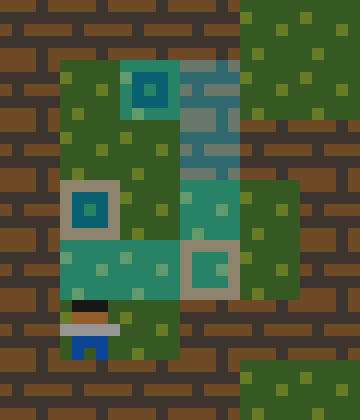
\includegraphics[width=\linewidth]{Images/firstScoreBestFS}
  		\caption{Example of distance between winning objects metric}
  		\label{Figure:bestFS1}
	\end{minipage}\hfill
	\begin{minipage}{0.45\textwidth}
		\centering
  		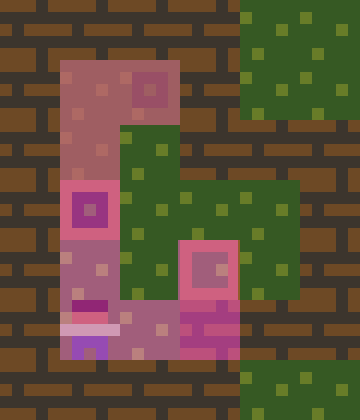
\includegraphics[width=\linewidth]{Images/secondScoreBestFS}
  		\caption{Example of distance between player and winning objects metric}
  		\label{Figure:bestFS2}
	\end{minipage}
\end{hcfigure}

These metrics works fine for all games where player is not one of the winning objects. When the player is one of the winning objects, the two metrics behaves in the same way. The player always tries to move towards the winning objects regardless of any other game objects. For example, \figref{lavaGame} shows a level from a game called LavaGame. LavaGame is a puzzle game where the goal is to make the player reach the exit. The path towards the exit is usually stuck by lava which can be destroyed by pushing a crate over it. According to the Lim et al. metrics, the player will try to move nearer to the exit by going left. This movement will not help the player to reach the exit, so the player will start wandering aimlessly trying to stumble across a movement sequence that can solve the level.

\gfigure{Example level from LavaGame showing the problem in the old metrics}{lavaGame}{width=3.0in}{Images/lavaGame}

Player's aim is to move crates towards the lava to unblock his path towards the exit. This aim is somehow explained in the game rules, so by further analysis the game rules we can know which objects need to be closer. Returning to our example about LavaGame, the game rules are stated in the following order:
\begin{center}{[> Player | Crate] -> [> Player | > Crate]}\end{center}
\begin{center}{[> Crate | Lava] -> [ \ \ \ \ | \ \ \ \ ]}\end{center}
The first rule says if there is a player and crate beside each other and the player moves toward it, the crate will also move. The second rule says if there is a crate and lava beside each other and the crate moves toward it, both crate and lava will be destroyed. In any proper game, rules must be applied before achieving the winning condition. Based on that fact, the distance between objects on the left hand side of the rules must be decreased. The relation between objects in the left hand side of the rules is captured by the Rule Analyzer Relations list for each game object. This distance is used as the new heuristic measure beside the original ones. The three metrics are given different weights and used as a new fitness function to evaluate game states. The weights are chosen by experimentation to ensure the best results.\\\par

The output of the automated player is essential in evaluating the level quality. Four different values are returned which capture the way the automated player plays the level. These four values are:
\begin{itemize} \itemsep0pt \parskip0pt \parsep0pt
	\item \textbf{The score for the best reached state so far:} The score is calculated using the first metric (Distance between winning objects). The best achieved score for all states is reported.
	\item \textbf{The movement sequence to reach the best state:} The automated player saves up all the movements that happen to reach each state and returns the sequence that leads to the best state.
	\item \textbf{The number of states explored while searching for the solutions:} The automated player saves the number of states that it explores before terminating.
	\item \textbf{The number of rules that the game engine applies to reach the best state:} With each movement, some rules may be applied by the game engine. The automated player saves this number for each state and returns the number associated with the best state.
\end{itemize}
The modified BestFS finds the solution faster than original one. More details will be explained in \chref{Chapter5}.\\\par

\subsubsection{Heuristic Measures}\seclbl{levelScoreEquation}
Heuristic measures are calculated using a weighted function of six attributes. The function is described as the following:
\begin{center}$F_{score} = 0.3 * P_{score} + 0.2 * L_{score} + 0.15 * N_{score} + 0.12 * B_{score} + 0.12 * R_{score} + 0.11 * E_{score}$\end{center}
where $P_{score}$ is the Playing Score, $L_{score}$ is the Solution Length Score, $N_{score}$ is the Object Number Score, $B_{score}$ is the Box Line Score, $R_{score}$ is the Applied Rule Score, and $E_{score}$ is the Exploration Score. The weights for each attribute are measured experimentally to reflect the importance of each features in the generated levels. The following points will further explain each of these scores.
\begin{itemize}
	\item \textbf{Playing Score ($P_{score}$):} Playing score is used to ensure level playability. Instead of using a boolean value for playable or not. A float value is assigned for how much the player is near the solution. The first output of the automated player is used for that purpose. Making the domain more continuous (using float) helps in measuring the percentage of the level playability instead of using it as a constraint.\\\par
	
	Based on the work by Nielsen et al.\cite{gvgpPerformanceProfiles} which proved that static players (Do Nothing players) score badly in all human crafted games. These bad scores prove that the Do Nothing players can be used as a measurement for game design. A score is calculated for the initial level state. This score is subtracted from the previous score to show how much improvement the automated player have done. The Playing Score can be expressed by the following equation:
	\begin{center}$ P_{score} = S_{play} - S_{nothing}$\end{center}
	where $S_{play}$ is the automated player score and $S_{nothing}$ is the Do Nothing player score.
	
	\item\textbf{Solution Length Score ($L_{score}$):} \figref{diffLevelsSokoban} shows that interesting levels usually have more steps than the trivial ones. The first idea is to compare the length of the best movement sequence with a target value. This idea will not work as expected because solution length depends on the size of the level. For example, \figref{sokobanLenghtArea} shows different levels from Sokoban and their corresponding solution length. Its obvious that the seconds level has longer solution because it has bigger area.
	
	\gfigure{Examples of two sokoban levels with different area and solution lengths}{sokobanLenghtArea}{width=4.5in}{Images/sokobanLenghtArea}
	
	From the previous example we can conclude that the solution length depends on the level area. Instead of using the solution length as the metric we used the ratio between the solution length and the level area. A mapping function is used to convert that number to a value in the range of [0, 1]. We analyzed 40 hand crafted levels with different area from 5 different games. A histogram is plotted for the ratio between the solution length and the level area and shown in \figref{solutionLengthHistogram}.
	
	\gfigure{Histogram for the ratio between the solution length and the level area}{solutionLengthHistogram}{width=5.5in}{Images/solutionLengthHistogram}
	
	The histogram seems to follow a Normal Distribution with $\mu = 1.221$ and $\sigma = 0.461$. Based on that, the Solution Length Score is expressed by the following equation:
	\begin{center}$L_{score} = Normal(\dfrac{L}{A}, 1.221, 0.461)$\end{center}
	where $Normal(ratio, \mu, \sigma)$ is a normal distribution function, $L$ is the solution length, and $A$ is the level area.
	
	\item \textbf{Object Number Score ($N_{score}$):} The Object Number Score is calculated by the following equation:
	\begin{center}$N_{score} = 0.4 * N_{rule} + 0.3 * N_{player} + 0.3 * N_{winning}$\end{center}
	where $N_{rule}$ is the Number of Rule Objects ratio, $N_{player}$ is the Number of Players value, and $N_{winning}$ is the Number of Winning Objects value.
	\begin{itemize}
		\item \textbf{Number of Rule Objects ($N_{rule}$):} In a good designed level, most of the rule objects should appear in the level to ensure there is a possibility of applying every rule. The number of times the object should appear in the level must be greater than or equal his minimum required number property from the Rule Analyzer. A ratio is calculated between the number of objects greater than their minimum required number property and the total number of the rule objects.
		\begin{center}$N_{rule} = \dfrac{N_{min}}{N_{max}}$\end{center}
		where $N_{min}$ is the number of objects greater than their minimum required number property and $N_{max}$ is the total number of the rule objects.
		\item \textbf{Number of Players ($N_{player}$):} The game should have only one player. If any level has a different value, the score will be zero.
		\begin{center}
		$N_{player}= \begin{cases}
		               1 & \text{one player object exists}\\
		               0 & \text{otherwise}
		           \end{cases}$
		\end{center}
		\item \textbf{Number of Winning Objects ($N_{winning}$):} The number of both winning objects should be equal, unless one of them have a "Create" behavior. Based on the previous condition, the score is set to either one or zero.
		\begin{center}
			$N_{winning}= \begin{cases}
			               1 & \ N_{winnObj1} == N_{winObj2} \text{ and no Create behavior}\\
			               1 & \text{Create behavior exists}\\
			               0 & \text{otherwise}
			           \end{cases}$
		\end{center}
		where $N_{winObj1}$ is the number of the first winning object and $N_{winObj2}$ is the number of the second winning object.
	\end{itemize}
	
	\item \textbf{Box Line Score ($B_{score}$):} It is similar to Taylor and Parberry\cite{sokobanLevelGenerationNew} metric to find the farthest state. This metric calculates the number of unrepeated moves found in the solution and divide it by the solution length. The following equation represents it:
	\begin{center}$B_{score} = \dfrac{L_{unique}}{L}$\end{center}
	where $L_{unique}$ is the number of unrepeated moves in the solution and $L$ is the solution length.
	
	\item \textbf{Applied Rule Score ($R_{score}$):} Good level design involves applying game rules for a number of times to solve any level. The ratio between the number of applied rules to the solution length should be used for indicting good level design. Exaggerating in applying the rules results in boring level. Same can be said for the very low amount of applying. \figref{sokobanRuleScore} shows two levels from Sokoban with different solutions. The left level needs to apply Sokoban's rule for one time to solve the level, while the right needs to apply Sokoban's rule with every single step.
	
	\gfigure{Example for two boring levels from Sokoban}{sokobanRuleScore}{width=4.5in}{Images/sokobanRuleScore}
	
	To find the best ratio between both, We analyzed 40 hand crafted levels from 5 different games. A histogram is plotted for the ratio between the number of applied rules and the solution length is shown in \figref{rulesSolutionLengthHistogram}.
	
	\gfigure{Histogram for the number of rules applied to the solution length}{rulesSolutionLengthHistogram}{width=5.5in}{Images/rulesSolutionLengthHistogram}
	
	Again the histogram seems to follow a Normal Distribution with $\mu = 0.417$ and $\sigma = 0.128$. Based on that the Applied Rule Score can be expressed by the following equation:
	\begin{center}$R_{score} = Normal(\dfrac{R_{applied} \pm R_{none}}{L}, 0.417, 0.128)$\end{center}
	where $Normal(ration, \mu, \sigma)$ is a normal distribution function, $R_{applied}$ is the number of applied rules, $R_{none}$ is the number of applied rules with no action associated, and $L$ is the solution length. The $R_{none}$ is used to decrease the normal distribution value according to amount of rules applied at the beginning of the game with no action associated to decrease them from happening.
	
	\item \textbf{Exploration Score ($E_{score}$):} The increase in the number of explored states by the automated player means that the current level is not obvious to be solved directly by the automated player heuristics. This does not mean exploring huge space without finding a solution is better than exploring small number of states with a solution. The following equation express this idea:
	\begin{center}
	$E_{score}= \begin{cases}
	               0.75 + \dfrac{N_{explored}}{N_{max}} & \text{solution exists}\\
	               0.5 & \text{no solution and }N_{explored} = N_{max}\\
	               0 & \text{no solution and }N_{explored} < N_{max}
	           \end{cases}$
	\end{center}
	where $N_{explored}$ is the number of explored states and $N_{max}$ is the maximum number of states the automated player can explore. The automated player has a fixed number of iterations to ensure fast execution.
\end{itemize}

\section{Rule Generation}
As stated in the previous chapters, Rule Generation is the most difficult task in PCG. This work explores the idea behind generating new rules for the Puzzle Script engine. Unlike the work by Lim et al.\cite{puzzleScriptGeneration}, we are exploring Puzzle Script rules without fixing a certain level or a winning condition. \figref{ruleGeneratorBlockDiagram} shows a high level block diagram for the system. The system is a bit similar to the level generation system as the level generation system is a module inside the whole system.

\gfigure{High level system block diagram for Rule Generation}{ruleGeneratorBlockDiagram}{width=5.8in}{Images/ruleGeneratorBlockDiagram}

The system starts by generating random rules for different games. These rules are analyzed using the same Rule Analyzer used in the Level Generation process. The object features with a level layout are fed to a Constructive Approach Level Generator. The generated rules and the resulted levels are subjected to an evaluator similar to the one used in the Level Generation process. The system evolves using the same GA operators from Lim et al. work\cite{puzzleScriptGeneration}. In the following subsections each module in the block diagram is discussed in details.

\subsection{Rule Generator}
Rule Generator is responsible for generating and evolving rules. Rule generator uses GA for the evolution process. It is the same system used by Lim et al.\cite{puzzleScriptGeneration} in his work.\\\\
\textbf{Chromosome Representation:} The chromosome represents a list of rules of maximum four and a minimum one plus a single winning condition. \\\\
\textbf{Genetic Operators:} Crossover and Mutation are used to evolve the rules. Crossover takes place only when the two chromosomes possess the same number of rules, the same number of tuples within each rule, and the same number of objects per tuple. There are two kinds of crossover that can take place:
\begin{itemize} \itemsep0pt \parskip0pt \parsep0pt
	\item \textbf{Hand Side Crossover:} Single point crossover is used to swap the whole right hand side between rules of different chromosomes.
	\item \textbf{Element Crossover:} Two point crossover is used to swap a single object from the first chromosome with the second one.
\end{itemize}

Mutation has no preconditions to take place except for a certain probability. There are five different mutation operators (mutators). Chromosomes are subjected to each one based on a certain probability. The five mutators are:
\begin{itemize} \itemsep0pt \parskip0pt \parsep0pt
	\item \textbf{Rule size mutator:} changes the number of rules either by adding an empty rule or removing a rule.
	\item \textbf{Object mutator:} changes a random object in a rule with any random object.
	\item \textbf{Direction mutator:} changes the direction of a random object in a rule. It also can add or remove a direction for a random object.
	\item \textbf{Tuple size mutator:} change the number of objects inside the tuple by either deleting a random object or adding a random object with a random direction.
	\item \textbf{Hand side swap mutator:} swaps the left hand side with the right hand side of a rule.
\end{itemize}

These operators are not used over the winning condition. The winning condition has a separate crossover and mutation operators. Crossover is done using two points crossover to swap one of the winning objects or the winning condition. Mutation replaces any of the winning objects with a random object or changes the winning condition to a random rule.\\\\
\textbf{Initial Population:} The population is initialized randomly using mutated versions of an empty rule.

\subsection{Rule Analyzer}
Rule Analyzer is responsible for understanding the generated rules by the Rule Generator. The same Rule Analyzer from \secref{ruleAnalyzer} is used here.

\subsection{Level Generator}
Level Generator is responsible for generating random levels for the generated rules. It uses the Constructive Approach algorithm described in \secref{constructiveApproach}.

\subsection{Rule and Level Evaluator}
Rule and Level Evaluator is responsible for giving a score for the generated games (rules and levels). It is a combination between the Level Evaluator from \secref{levelEvaluator} and Lim et al.\cite{puzzleScriptGeneration} Evaluator. The weights are measured experimentally to ensure the best results. The game evaluation score can be expressed by the following equation:
\begin{center}
$RL_{score} = 0.5 * L_{score} + 0.5 * R_{score}$
\end{center}
where $L_{score}$ is the level score and $R_{score}$ is the rule score.

\subsubsection{Level Score}
It uses the automated player described in \secref{automatedPlayer} to give each generated level a score and the best scored level is the selected one. The level score is calculated using the same equation in \secref{levelScoreEquation} except for the Playability Score. Instead of using a range of values, It is just indicates if it is playable or not to point out the importance of finding playable rules.

\subsubsection{Rule Score}
It is divided into 2 different parts rule heuristics score and rule validity score. The weights are measured experimentally to ensure the best results. The rule score can be expressed by the following equation:
\begin{center}
$R_{score} = 0.6 * H_{score} + 0.4 * V_{score}$
\end{center}
where $H_{score}$ is the rule heuristic score and $V_{score}$ is the rule validity score.\\\\
\textbf{Rule Heuristics Score ($H_{score}$):} It is similar to Lim et al.\cite{puzzleScriptGeneration} heuristics. It is a group of heuristics that ensures higher chance of playability for the generated games. The Rule Heuristic Score can be expressed by the following equation:
\begin{center}
$H_{score} = \dfrac{1}{8} * (P_{score} + C_{score} + U_{score} + W_{score} + WO_{score} + PL_{score} + M_{score} + D_{score})$
\end{center}
where $P_{score}$ is the player exists score, $C_{score}$ is the critical path exists score, $U_{score}$ is the useless objects score, $W_{score}$ is the winning condition validity score, $WO_{score}$ is the winning object in the rules score, $L_{score}$ is the player in LHS score, $M_{score}$ is the player movement score, and $D_{score}$ is the direction consistency score.
\begin{itemize} \itemsep0pt \parskip0pt \parsep0pt
	\item \textbf{Player exists score ($P_{score}$):} It ensures that a player exists in any of the game rules. The player object must exist in the rules to have some game interaction. It can be expressed by the following equation:
	\begin{center}
		$P_{score}= \begin{cases}
		               1 & \text{player exists in the rules}\\
		               0 & \text{otherwise}
		           \end{cases}$
		\end{center}
	\item \textbf{Critical path exists score ($C_{score}$):} It ensures the existence of a path between the player object and at least one of the winning objects in the Relations list. Having a path ensures that the game can be finished by moving with the player. It can be expressed by the following equation:
	\begin{center}
	$C_{score}= \begin{cases}
	               1 & \text{citical path exists}\\
	               0 & \text{otherwise}
	           \end{cases}$
	\end{center}
	\item \textbf{Useless objects score ($U_{score}$):} The amount of useless objects found in the game rules. Useless objects are rule objects that are neither connected to a player or a winning condition in the Relations list. Useless objects are not affected by any player action so the score is inversely proportional to their number. The score can be expressed by the following equation:
	\begin{center}
	$U_{score} = \dfrac{1}{N_{useless} + 1}$
	\end{center}
	where $N_{useless}$ is the number of useless objects.
	\item \textbf{Winning condition validity score($W_{score}$):} The winning objects should have some features to ensure game playability. These features differ according to the winning condition. No rule requires at least one of the winning object having a Delete, Move, or Teleport behavior, while other winning rules (All and Some) requires Create, Move, or Teleport behavior. This score can be expressed by the following equation:
	\begin{center}
	$W_{score}= \begin{cases}
	               1 & \text{winning object have one of the required features}\\
	               0 & \text{otherwise}
	           \end{cases}$
	\end{center}	
	\item \textbf{Winning object in the rules score ($WO_{score}$):} At least one of the two winning objects should appear in any rule. This score can be expressed using the following equation:
	\begin{center}
	$WO_{score}= \begin{cases}
	               1 & \text{at least one winning object exists in the rules}\\
	               0 & \text{otherwise}
	           \end{cases}$
	\end{center}
	\item \textbf{Player in LHS score ($PL_{score}$):} Player should exists on the left hand side of at least one rule. This score can be expressed by the following equation:
	\begin{center}
	$PL_{score}= \begin{cases}
	               1 & \text{player exists in LHS of at least one rule}\\
	               0 & \text{otherwise}
	           \end{cases}$
	\end{center}	
	\item \textbf{Player Movement ($M_{score}$):} Player should have at least one movement action associated with it in any rule to affect other game objects. This score can be expressed by the following equation:
	\begin{center}
	$M_{score}= \begin{cases}
	               1 & \text{player movement exists}\\
	               0 & \text{otherwise}
	           \end{cases}$
	\end{center}	
	\item \textbf{Direction consistency ($D_{score}$):} Rules should have the same movement action across the whole rule to ensure human playability. The score is inversely proportional to the number of different movements in the rules. This score can be expressed by the following equation:
	\begin{center}
	$D_{score} = \dfrac{1}{D_{unique}}$
	\end{center}
	where $D_{unique}$ is the average number of unique movement for all rules.
\end{itemize}
\textbf{Rule Validity Score ($V_{score}$):} It ensures that no errors are found in the generated rules. Errors can be detected from Puzzle Script engine during the compilation process. This score can be expressed using the following equation:
\begin{center}
$V_{score}= \begin{cases}
               1 & \text{no errors}\\
               0 & \text{otherwise}
           \end{cases}$
\end{center}